\documentclass[11pt, onecolumn]{article}
% \setlength{\columnsep}{0.2cm}

\usepackage{amssymb}
\usepackage{amsmath}
\usepackage[a4paper, margin=1.5cm]{geometry}
%\usepackage{mathtools}
\usepackage{graphicx}

\usepackage{color}
\usepackage[usenames,dvipsnames,svgnames,table]{xcolor}

\usepackage[colorlinks=true,linkcolor=blue, citecolor=BlueGreen]{hyperref}
%\hypersetup{ pdfborder = {0 0 0}}

\usepackage[parfill]{parskip}
\usepackage{lscape}

\usepackage{xspace}

\usepackage{fancyhdr}
\pagestyle{fancy}
\lhead{ }
\rhead{\naf documentation}

%%%%%%%%%%%%%%%%%%%%%%%%

\title{\naf (New Agent-based model for Flu) Documentation}
\author{David Champredon}

%%%%%%%%%%%%%%%%%%%%%%%%

\newcommand{\ttt}[1]{\texttt{#1}}
\newcommand{\one}[1]{\textbf{\large{1}}_{#1}}
\newcommand{\warning}[1]{\textbf{\textcolor{OrangeRed}{#1}}}
\newcommand{\note}[1]{\textit{\textcolor{Grey}{Note: #1}}}
\newcommand{\eg}{\textit{e.g.}}
\newcommand{\ie}{\textit{i.e.}}
\newcommand{\naf}{\textsf{NAF}\xspace}


%%%%%%%%%%%%%%%%%%%%%%%%
%%%%%%%%%%%%%%%%%%%%%%%%
%%%%%%%%%%%%%%%%%%%%%%%%
%%%%%%%%%%%%%%%%%%%%%%%%

\begin{document}
\maketitle

\vspace{1cm}

\tableofcontents


\section{Introduction}

\section{Tests performed}

\begin{itemize}
\item \textbf{SEIR ODEs.} One unique spatial location, homogeneous mixing. Compare solutions of the standard ODE model with \naf. Test passed, see figure xxx.
\item \textbf{Migrations between social places.} Only two social places, no epidemic. Check if migrations occur as specified by schedule. Test passed. 
\end{itemize}


\section{Literature on influenza disease parameters}

\subsection{Natural history}

\textbf{Incubation.} Typically 1-4 days.

\textbf{Viral shedding.} Typically 1 day before symptoms appear. Could be sooner for young children. Shedding sharply reduces after 3-5 days, but could take much longer in young children (up to 10 days after onset). 

\textbf{Recovery.} Typically after 3-7 days after onset.


\subsection{Viral shedding}

Shedding can start about 1 day before symptoms onset, but can even be earlier among young children \cite{CDC:2011wq}. Shedding lasts for several days but is usually sharply reduced by day 3-5 after onset \cite{CDC:2011wq}. The decrease rate is exponential and weak patients experience a slower and longer decrease \cite{Lee:2009dc}.

\begin{figure}[!ht]
\centering
    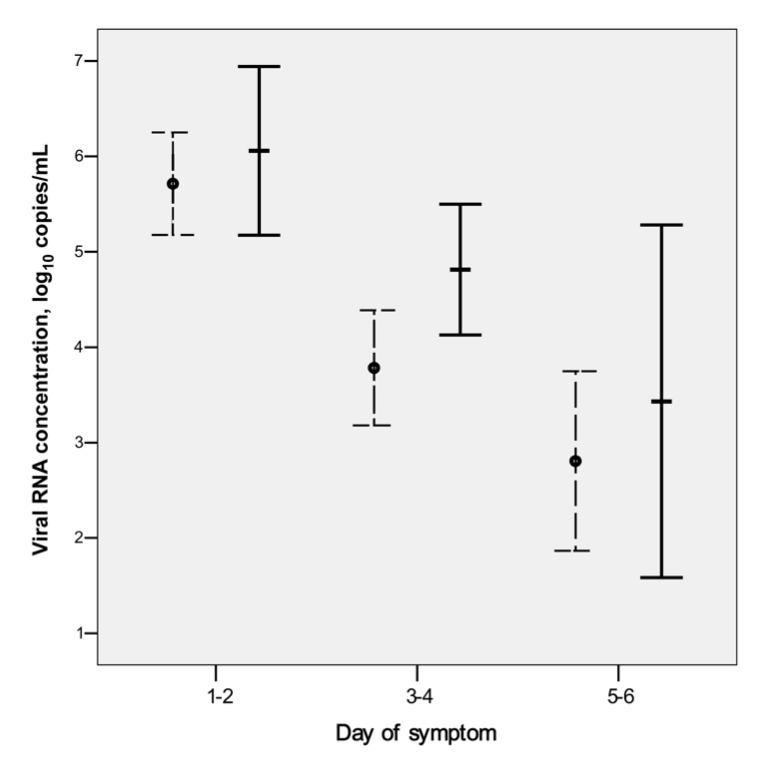
\includegraphics[angle=0,width=0.6\textwidth]{figures/VL_Lee.png}
\caption{Temporal evolution of viral load. Solid lines represent patients with major commorbidities, dashed those without. Source: Lee 2009 \cite{Lee:2009dc}}
\label{fig:VL_Lee}
\end{figure}


\subsection{Hospitalization}

Large majority of children hospitalizations last less than 2 days. Median 3-4 days. Hospitalization mostly occur in young children with pre-existing condition.

Fatality rate in hospital is typically 1-3\% in wealthy countries, but is higher among elderly (6-30\%, but this estimates include poor countries \cite{Wong:2015bb}.



\subsection{Antiviral Treatments}

Ressources:
\begin{itemize}
\item  CDC recommendations offer a nice overview \cite{CDC:2011wq}.
\item Reviews: Ebell\cite{Ebell:2014ic},  Jefferson 2014 \cite{Jefferson:2014ei}, Jackson 2011 \cite{Jackson:2011ff}
\item 
\end{itemize}

Four drugs: 
\begin{itemize}
\item Amantadine and rimantadine: for influenza A only, experience drug resistance.
\item Oseltamivir, Zanamivir: for both influenza A and B, drug resistance rare.
\end{itemize}

Overall, when used on patients already infected, treatment reduces marginally symptoms duration and does not reduce the risk of hospitalization \cite{Ebell:2014ic,Jefferson:2014ei}. 
If administrated within 2 days of onset: reduce duration of uncomplicated illness by 1 day.
If administrated within 1 day of onset: reduce duration of uncomplicated illness by 3.5 days among young children($<3$ years-old) \cite{CDC:2011wq}.

Treatment reduces amount of viral shedding (by how much?) but it's not clear if it reduces the shedding duration.

It is not clear if treatment reduces the risk of severe complications.

Post-exposure chemoprophylaxis is effective at preventing illness (may still be asymptomatic?): 70-90\% reduction in households context. Typical treatment duration: 10 days after most recent contact known \cite{CDC:2011wq}.

Pre-exposure chemoprophylaxis is effective at preventing illness: 80-90\%. Duration of treatment can be as long as 1 month. But because of resistance concerns, pre-exposure chemoprophylaxis is used only for persons at very high risk \cite{CDC:2011wq}. 

Adherence to treatment -- especially for long treatment durations -- is an issue because of side effects.



\subsection{Vaccination}

Influenza vaccine seems to be effective at reducing disease symptoms and severity, if infected later (at least 10 days later?).




%\begin{figure}[!ht]
%\centering
%    \includegraphics[angle=0,width=0.9\textwidth]{figures/hazard_death.pdf}
%\caption{Death hazard. The red dot represents the age of HIV acquisition. Vertical dashed lines are set at 5, 7 and 10 years after HIV acquisition.}
%\label{fig:deathHazard}
%\end{figure}


\bibliography{papers}
\bibliographystyle{plain}

\end{document}




